% document's head

\begin{center}
    \LARGE \textsc{Лабораторная работа № 6.11.1} \\
    \vspace{3 mm}
    \large Закон Кюри-Вейсса и обменное взаимодействие в ферромагнетиках
\end{center}

% \hrule

\phantom{42}

\begin{flushright}
    \begin{tabular}{rr}
    % written by:
        % \textbf{Источник}: 
        % & \href{__ссылка__}{__название__} \\
        % & \\
        % \textbf{Лектор}: 
        % & _ФИО_ \\
        % & \\
        \textbf{Автор работы}: 
        & Хоружий Кирилл \\
        & \\
    % date:
        \textbf{От}: &
        \textit{\today}\\
    \end{tabular}
\end{flushright}

\thispagestyle{empty}

\vspace{10mm}


\subsection*{Цель работы}
\begin{enumerate*}
    \item Исследовать температурную зависимость проводимости полупроводника.
    \item Определить ширину запрещенной зоны полупроводника из полученной зависимости.

\end{enumerate*}


\vfill

\begin{figure}[h]
    \centering
    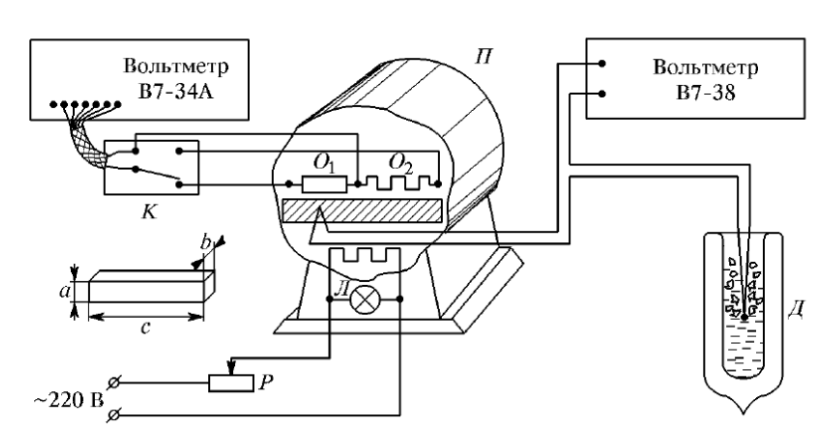
\includegraphics[width=0.5\textwidth]{exp.png}
    \caption{Схема установки}
    \label{fig:exp}
\end{figure}


\subsection*{Оборудование}

\begin{itemize}
    \item электронагревательная печь П;
    \item вольтметр В7-34А (погрешность примем $5\cdot10^{-4}$ кОм) 
    \item Полупроводниковый образец в форме параллелепипеда: $4.0 \times 4.0 \times 39$ (в мм);
    \item  Медный образец -- тонкая проволока длиной $l = 14$ м диаметра $d = 0.07$ мм;
    \item термопара.
\end{itemize}




